% Created 2018-10-22 Mon 12:42
% Intended LaTeX compiler: pdflatex
\documentclass[presentation]{beamer}
\usepackage[utf8]{inputenc}
\usepackage[T1]{fontenc}
\usepackage{graphicx}
\usepackage{grffile}
\usepackage{longtable}
\usepackage{wrapfig}
\usepackage{rotating}
\usepackage[normalem]{ulem}
\usepackage{amsmath}
\usepackage{textcomp}
\usepackage{amssymb}
\usepackage{capt-of}
\usepackage{hyperref}
\usepackage{tabu}
\usepackage{minted}
\usepackage[english, ngerman]{babel}
\hypersetup{pdfauthor="Vasilij Schneidermann", pdftitle="Krypto knacken für Anfänger", colorlinks, linkcolor=, urlcolor=blue}
\setminted{fontsize=\footnotesize,escapeinside=@@}
\usetheme{Rochester}
\usecolortheme[RGB={87,83,170}]{structure}
\author{Vasilij Schneidermann}
\date{Oktober 2018}
\title{Krypto knacken für Anfänger}
\uselanguage{German}
\languagepath{German}
\hypersetup{
 pdfauthor={Vasilij Schneidermann},
 pdftitle={Krypto knacken für Anfänger},
 pdfkeywords={},
 pdfsubject={},
 pdfcreator={Emacs 26.1 (Org mode 9.1.9)}, 
 pdflang={Ngerman}}
\begin{document}

\maketitle
\begin{frame}{Outline}
\tableofcontents
\end{frame}

\AtBeginSection{\frame{\sectionpage}}
\shorthandoff{"}

\section{Intro}
\label{sec:org78160f1}

\begin{frame}[label={sec:org36f2fcc}]{Sprecher}
\begin{itemize}
\item Vasilij Schneidermann, 26
\item Software-Entwickler bei \href{https://www.bevuta.com/en/}{bevuta IT GmbH}
\item mail@vasilij.de
\item \url{https://github.com/wasamasa}
\item \url{http://emacshorrors.com/}
\item \url{http://emacsninja.com/}
\end{itemize}
\end{frame}

\begin{frame}[label={sec:org74fa714}]{Motivation}
\begin{itemize}
\item Kryptographie ist nicht mehr wegzudenken
\item Viele Exploits mit einfallsreichen Namen (ROBOT, KRACK, EFAIL)
\item Viele Papers über Side-Channel-Angriffe (Meltdown, Spectre, TLBleed,
Foreshadow)
\item Dennoch: Viele Menschen ignorieren Krypto oder beschäftigen sich
lieber mit Kryptowährungen
\item Wie steigt man in das Thema ein?
\item Wie schwierig ist es wirklich?
\end{itemize}
\end{frame}

\begin{frame}[label={sec:orgb4ef2cd}]{Kontext}
\begin{itemize}
\item Suche nach interessanten Programmierübungen
\item \url{https://cryptopals.com/}
\begin{itemize}
\item Interessante Claims (Minimum an Mathematik, realistische Angriffe)
\item Gutes Design, aufeinander aufbauend
\item Viele Felder abgedeckt (symmetrische/asymmetrische Krypto,
Signaturen, PRNG, Hashes, Zero-Knowledge Proofs,
Protokolle/Handshakes)
\item Programmiersprache ist irrelevant
\item Offline lösbar (ursprünglich via E-Mail)
\item Maximale Freiheit gegeben
\end{itemize}
\end{itemize}
\end{frame}

\begin{frame}[label={sec:org997598e}]{Grundlagen}
\begin{itemize}
\item Confidentiality, Integrity, Authenticity
\item Symmetrische, asymmetrische Verschlüsselung
\item Plaintext, Ciphertext
\item Key, IV, Nonce
\item Block Cipher, Stream Cipher
\end{itemize}
\end{frame}

\section{Ausgewählte Angriffe}
\label{sec:org6b83c5c}

\begin{frame}[label={sec:org890a129}]{Kandidaten}
\begin{itemize}
\item Crack an MT19937 seed
\item Single-byte XOR cipher
\item CBC bitflipping attacks
\item Break “random access read/write” AES CTR
\item Compression Ratio Side-Channel Attacks
\end{itemize}
\end{frame}

\begin{frame}[label={sec:org96441e4}]{Verwendete Programmiersprache}
\begin{itemize}
\item Ich habe mich für Ruby entschieden
\begin{itemize}
\item Ausdrucksstark
\item Umfangreiche Standardbibliothek
\item Erfüllt alle Vorbedingungen (OpenSSL, Bignums)
\item Gelegenheit meine Ruby-Skills aufzubessern
\end{itemize}
\end{itemize}
\end{frame}

\begin{frame}[label={sec:orga4d111c}]{Crack an MT19937 seed}
\begin{itemize}
\item Involviert (noch) keine Krypto
\item MT19937 ist ein populärer PRNG
\item Manche Leute nutzen es für Krypto\ldots{}
\item Manche Leute seeden es mit der aktuellen Zeit\ldots{}
\item Gegeben sei der erste MT19937-Output mit der aktuellen Zeit von vor
wenigen Minuten als Seed
\item Wie knackt man den Seed?
\end{itemize}
\end{frame}

\begin{frame}[fragile,label={sec:org6d0ca3b}]{Crack an MT19937 seed}
 \begin{minted}[]{ruby}
def random_number(seed)
  Random.new(seed).rand(2**32)
end

now = Time.now.to_i
seed = now - 123
rng_output = random_number(seed)
\end{minted}
\end{frame}

\begin{frame}[label={sec:orgf343eff}]{Crack an MT19937 seed}
\begin{itemize}
\item Ein PRNG generiert eine eindeutige Zahlenfolge für einen Seed
\item Wenn man den gleichen Seed verwendet, erhält man die gleiche
Zahlenfolge
\item Idee: Alle möglichen Zeitstempel als Seed probieren, testen ob die
erste generierte Zahl übereinstimmt
\end{itemize}
\end{frame}

\begin{frame}[fragile,label={sec:org5973096}]{Crack an MT19937 seed}
 \begin{minted}[]{ruby}
def crack_it(start_time, rng_output)
  seed = start_time
  loop do
    return seed if random_number(seed) == rng_output
    seed -= 1
  end
end

puts "Predictable seed: #{seed}, output: #{rng_output}"
puts "Cracked seed: #{crack_it(now, rng_output)}"
\end{minted}
\end{frame}

\begin{frame}[label={sec:org5c04737}]{Crack an MT19937 seed}
\begin{itemize}
\item Aufwand: Vernachlässigbar
\item Passiert häufiger als man denkt: \url{https://arxiv.org/abs/1802.03367}
\item Workaround: Niemals mit erratbaren Daten seeden, CSPRNG vom
Betriebssystem verwenden (gute Bibliotheken tun das von Haus aus)
\item Kombination vieler Entropiequellen ist beliebt (PID,
systemspezifische Daten, etc.), aber nicht viel besser:
\url{https://blog.cr.yp.to/20140205-entropy.html}
\end{itemize}
\end{frame}

\begin{frame}[label={sec:org0733f6b}]{Single-byte XOR cipher}
\begin{itemize}
\item Moderne Variante der Caesar-Verschlüsselung
\item Jedes Byte vom Plaintext wird mit einem geheimen Byte durch den
XOR-Operator kombiniert
\item XOR ist umkehrbar: \(x \oplus y = z, z \oplus y = x, z \oplus x = y\)
\item Gegeben sei ein auf diese Weise verschlüsselter Text auf Englisch
\item Wie knackt man diesen Text?
\end{itemize}
\end{frame}

\begin{frame}[fragile,label={sec:org4801c6f}]{Single-byte XOR cipher}
 \begin{minted}[]{ruby}
ENGLISH_HISTOGRAM = {
  ' ' => 0.14,
  :other => 0.09,
  'e' => 0.12,
  't' => 0.09,
  'a' => 0.08,
  'o' => 0.07,
  'i' => 0.06,
  'n' => 0.06,
  # ...
}

def frequencies(string)
  result = Hash.new { |h, k| h[k] = 0 }
  total = string.length
  string.each_char { |char| result[char] += 1 }
  result.each { |k, v| result[k] = v.to_f / total }
  result
end
\end{minted}
\end{frame}

\begin{frame}[fragile,label={sec:org49881d1}]{Single-byte XOR cipher}
 \begin{minted}[]{ruby}
def chi_squared(hist1, hist2)
  score = 0
  hist1.each do |k, v1|
    v2 = hist2[k] || 0
    next if v1.zero?
    score += (v1 - v2)**2 / v1
  end
  score
end

def english_score(string)
  return 0 unless string.ascii_only?
  input = string.downcase.tr('^ a-z', '.')
  histogram = frequencies(input)
  histogram[:other] = histogram['.'] || 0
  histogram.delete('.')
  score = 1 / chi_squared(ENGLISH_HISTOGRAM, histogram)
  score *= 2 if histogram[:other] < 0.05
  score
end
\end{minted}
\end{frame}

\begin{frame}[fragile,label={sec:org6af65bc}]{Single-byte XOR cipher}
 \begin{minted}[]{ruby}
best_score = 0
best_solution = ''

(0..255).each do |key|
  solution = str(xor_buffer_with_byte(CIPHERTEXT, key))
  score = english_score(solution)
  if score > best_score
    best_score = score
    best_solution = solution
  end
end

puts "score: #{best_score}"
puts best_solution
\end{minted}
\end{frame}

\begin{frame}[label={sec:org4ad62f3}]{Single-byte XOR cipher}
\begin{itemize}
\item Größte Herausforderung: Brauchbare Scoring-Funktion schreiben
\item Verschlüsselung mit längeren Schlüsseln lassen sich ähnlich knacken
\item Es gibt kaputte Krypto-Systeme die auf diese Schwierigkeitsstufe
zurückfallen
\end{itemize}
\end{frame}

\begin{frame}[fragile,label={sec:org0458b8c}]{CBC bitflipping attacks}
 \begin{itemize}
\item Diese Übung nutzt nicht trivial knackbare Krypto (AES)
\item ECB wird nicht mehr empfohlen, deswegen wird hier CBC genutzt
\item Angenommen ein Angreifer findet einen mit AES-CBC verschlüsselten
Cookie der nach \texttt{comment=1234567890\&uid=3} aussieht
\item Der Angreifer möchte diesen Cookie so bearbeiten, dass \texttt{uid=0} drin
steht um Admin zu werden
\item Es ist nicht möglich für den Angreifer den Cookie zu entschlüsseln,
bearbeiten und erneut verschlüsseln (da Schlüssel und IV unbekannt)
\item Was passiert wenn man den Ciphertext direkt bearbeitet?
\end{itemize}
\end{frame}

\begin{frame}[fragile,label={sec:orgfaf3fbc}]{CBC bitflipping attacks}
 Modifikation: Erstes Byte wurde mit zufälligem Byte mit XOR kombiniert

\begin{minted}[]{text}
 regular ciphertext: @\textcolor{blue}{24}@fe5dcfa80f182d3e1ee5f486723e9b33516b7a2846b1..
tampered ciphertext: @\textcolor{blue}{66}@fe5dcfa80f182d3e1ee5f486723e9b33516b7a2846b1..
  regular plaintext: @\textcolor{red}{636f6d6d656e743d3132333435363738}@@\textcolor{blue}{39}@30267569643d33
 tampered plaintext: @\textcolor{red}{06ef88d48792df331838931d121fca22}@@\textcolor{blue}{7b}@30267569643d33

0x24 ^ 0x66 == 0x42
0x39 ^ 0x7b == 0x42
\end{minted}

Resultat: Erster Block ist komplett anders, erstes Byte vom zweiten
Block wurde auf die gleiche Weise manipuliert
\end{frame}

\begin{frame}[label={sec:org2b74a38}]{CBC bitflipping attacks}
\begin{figure}[htbp]
\centering
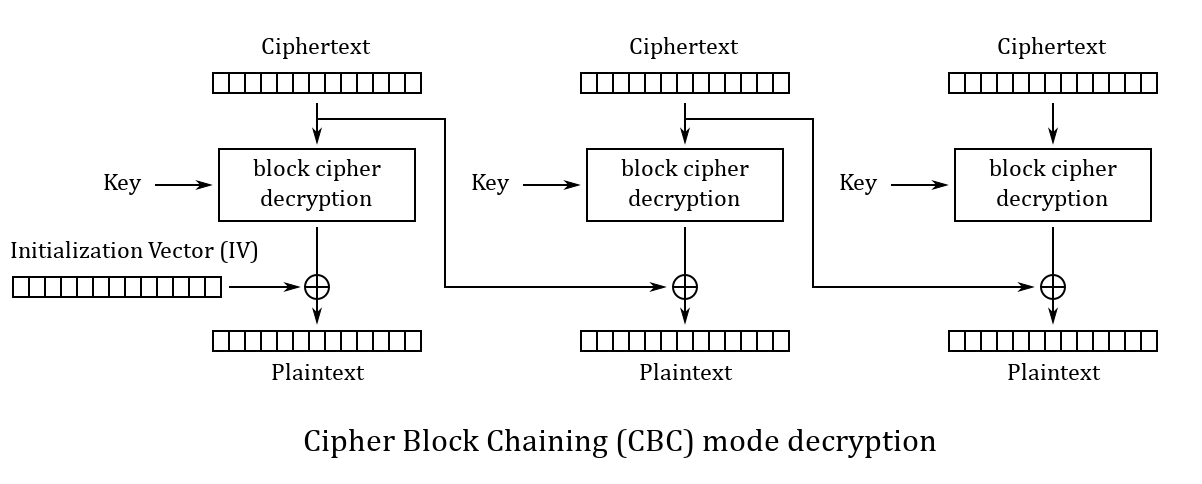
\includegraphics[width=.9\linewidth]{./img/cbc_decryption.png}
\caption{Quelle: Wikipedia}
\end{figure}
\end{frame}

\begin{frame}[fragile,label={sec:orga3a0235}]{CBC bitflipping attacks}
 \begin{minted}[]{ruby}
KEY = random_bytes(16)
IV = random_bytes(16)
PLAINTEXT = 'comment=1234567890&uid=3'
CIPHERTEXT = aes_cbc_encrypt(PLAINTEXT.bytes, KEY, IV)

def check(ciphertext)
  plaintext = str(aes_cbc_decrypt(ciphertext, KEY, IV))
  params = decode_query_string(plaintext)
  uid = params['uid']
  puts "checking #{plaintext.inspect}..."
  raise 'invalid string' unless uid
  uid.to_i
end
\end{minted}
\end{frame}

\begin{frame}[fragile,label={sec:orge0e1c5d}]{CBC bitflipping attacks}
 \begin{minted}[]{ruby}
tampered_byte = '3'.ord ^ '0'.ord
tampered = CIPHERTEXT.clone
tampered[7] ^= tampered_byte

puts "regular UID: #{check(CIPHERTEXT)}"
puts "tampered UID: #{check(tampered)}"
\end{minted}
\end{frame}

\begin{frame}[label={sec:org10b07d3}]{CBC bitflipping attacks}
\begin{itemize}
\item Nicht nur CBC ist von diesem Verhalten betroffen (bei CTR wird der
gleiche Block manipuliert)
\item Lösung: Cookies signieren und Signatur verifizieren, bei ungültiger
Signatur den Cookie nicht nutzen
\item Schlechte Lösung: Prüfsumme hinzufügen und überprüfen
\item Alternative: Verschlüsselung mit integrierter Authentication nutzen
(z.B. AES-GCM)
\end{itemize}
\end{frame}

\begin{frame}[fragile,label={sec:org7e62738}]{Break “random access read/write” AES CTR}
 \begin{itemize}
\item Erneut AES, diesmal mit Stream-Cipher
\item Angenommen ein Angreifer fängt eine mit AES-CTR verschlüsselte
Nachricht ab
\item Diese Nachricht stammt von einer Web-Anwendung die es Usern
ermöglicht verschlüsselte Nachrichten zu editieren
\item Es wird eine Eigenschaft von CTR für effizientes Editieren
ausgenutzt (damit nur der nötige Bruchteil der Nachricht ersetzt
werden muss)
\item Der Angreifer hat Zugriff auf einen interessanten API-Call welcher
einen neuen Ciphertext zurückgibt:
\texttt{/edit?ciphertext=...\&offset=...\&newtext=...}
\end{itemize}
\end{frame}

\begin{frame}[fragile,label={sec:org89bbe34}]{Break “random access read/write” AES CTR}
 \begin{minted}[]{ruby}
KEY = random_bytes(16)
NONCE = random_bytes(16)
CIPHERTEXT = aes_ctr_encrypt(PLAINTEXT, KEY, NONCE)

def edit_internal(ciphertext, key, nonce, offset, newtext)
  decrypted = aes_ctr_decrypt(ciphertext, key, nonce)
  newtext.each_with_index { |byte, i| decrypted[offset + i] = byte }
  aes_ctr_encrypt(decrypted, key, nonce)
end

def edit(ciphertext, offset, newtext)
  edit_internal(ciphertext, KEY, NONCE, offset, newtext)
end
\end{minted}
\end{frame}

\begin{frame}[label={sec:org519b225}]{Break “random access read/write” AES CTR}
\begin{figure}[htbp]
\centering
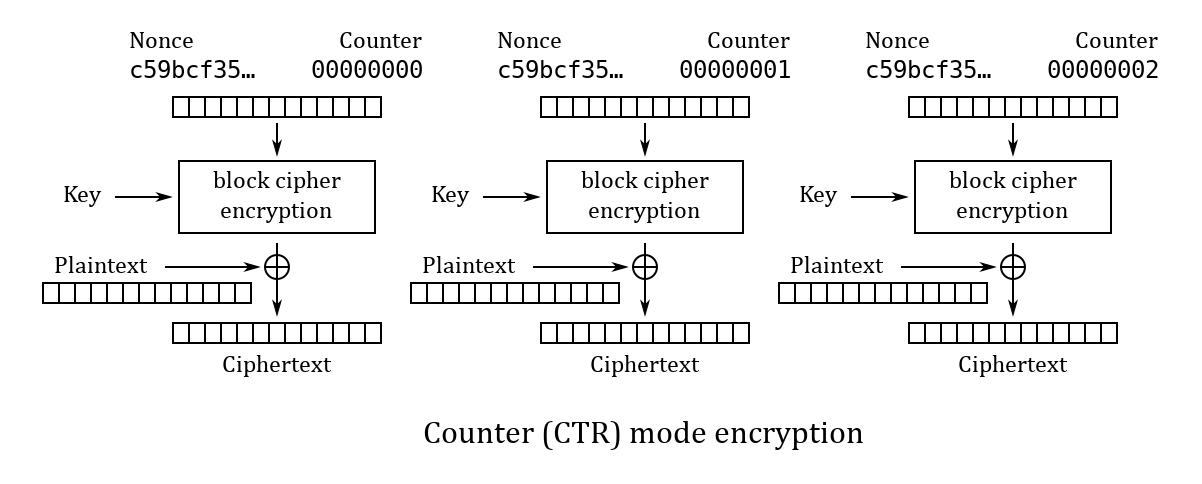
\includegraphics[width=.9\linewidth]{./img/ctr_encryption.png}
\caption{Quelle: Wikipedia}
\end{figure}
\end{frame}

\begin{frame}[label={sec:org1b30ceb}]{Break “random access read/write” AES CTR}
\begin{itemize}
\item Deutlich einfachere Transformation als bei CBC
\item Plaintext wird mit XOR mit verschlüsseltem Keystream kombiniert
\item Der Keystream ist mit einem Nonce parametrisiert
\item \(P_u \oplus E(k, K, N)\)
\item Wenn der Angreifer einen ihm bekannten Ciphertext mit dem
existierenden kombiniert, passiert folgendes:
\item \(P_u \oplus E(k, K, N) \oplus P_k \oplus E(k, K, N) = P_u \oplus P_k\)
\item Der Angreifer kennt seinen eigenen Plaintext, aber nicht den der
zu entschlüsselnden Nachricht
\item \(P_u \oplus P_k \oplus P_k = P_u\)
\end{itemize}
\end{frame}

\begin{frame}[fragile,label={sec:orgfff157f}]{Break “random access read/write” AES CTR}
 \begin{minted}[]{ruby}
random_message = random_bytes(ciphertext.length)
edited_message = edit(ciphertext, 0, random_message)
puts str(xor_buffers(xor_buffers(ciphertext, edited_message),
                     random_message))
\end{minted}
\end{frame}

\begin{frame}[fragile,label={sec:orgb77955a}]{Break “random access read/write” AES CTR}
 \begin{itemize}
\item Bonus: \texttt{/edit} erlaubt den Text Byte für Byte zu erraten
\item Angenommen der Angreifer vergleicht den editierten Ciphertext mit
dem ursprünglichen
\item Sind die Inhalte verschieden, werden die Ciphertexts auch
verschieden sein
\item Sind die Inhalte gleich, werden die Ciphertexts auch gleich sein
\item Wenn der Angreifer durch Zufall einen Edit gefunden bei dem der
gleiche Ciphertext zurückgegeben wird, hat er einen Teil des
Plaintexts erraten
\item Kleinstmöglicher Edit: 1 Byte
\item 1 Byte kann mit maximal 256 Edits erraten werden
\item Offset inkrementieren und das nächste Byte erraten
\end{itemize}
\end{frame}

\begin{frame}[fragile,label={sec:org50636e0}]{Break “random access read/write” AES CTR}
 \begin{minted}[]{ruby}
def guess_byte(ciphertext, offset)
  (0..127).each do |byte|
    return byte if ciphertext == edit(ciphertext, offset, [byte])
  end
  raise "couldn't guess byte"
end

ciphertext.size.times { |i| print guess_byte(ciphertext, i).chr }
\end{minted}
\end{frame}

\begin{frame}[label={sec:orga01e50d}]{Break “random access read/write” AES CTR}
\begin{itemize}
\item Ursache: Nonce wird wiederverwendet, wenn man das vermeidet ist der
Keystream ein anderer und der Angriff ist nicht mehr erfolgreich
\item Bonus: Möglichst wenig Informationen leaken, exzessive Zugriffe
loggen und blockieren
\item Gedankenexperiment: Was wäre wenn jemand diese Eigenschaft von CTR
auf FDE anwendet?
\end{itemize}
\end{frame}

\begin{frame}[label={sec:orge65eeb9}]{Compression Ratio Side-Channel Attacks}
\begin{itemize}
\item Side-Channel-Angriff, umgeht Krypto vollständig
\item Angenommen der Angreifer ist MITM, fängt HTTP-Nachrichten ab und
kann zu diesen neuen Text hinzufügen bevor sie durchgereicht werden
\item Der Angreifer möchte den Cookie im HTTP-Header erraten
\item Das ist möglich wenn die Nachricht vor der Verschlüsselung
komprimiert wird und man auf die Größe der Nachricht prüft
\end{itemize}
\end{frame}

\begin{frame}[fragile,label={sec:org5a61585}]{Compression Ratio Side-Channel Attacks}
 \begin{itemize}
\item Bei Kompression werden wiederkehrende Zeichenketten gefunden und mit
einer kürzeren ersetzt
\item Angenommen wir komprimieren einen Text der \texttt{sessionid=abcdef}
beinhaltet, dann würde dieser Text etwas besser komprimiert wenn
danach ein \texttt{sessionid=a} folgt
\item Würde stattdessen \texttt{sessionid=b} folgen, würde der Text etwas
schlechter komprimiert
\item Die Unterschiede werden üblicherweise in Bits gemessen, oft beträgt
der Unterschied aber mehr als ein Byte
\item Oracle: Ein Mechanismus der dem Angreifer ein Stück Information
verrät
\end{itemize}
\end{frame}

\begin{frame}[fragile,label={sec:org829f8a7}]{Compression Ratio Side-Channel Attacks}
 \begin{minted}[]{ruby}
def format_request(input)
  "POST / HTTP/1.1
Host: example.com
Cookie: sessionid=#{SESSIONID}
Content-Length: #{input.length}
#{input}
"
end

def oracle(input)
  key = random_bytes(16)
  nonce = random_bytes(16)
  payload = compress(format_request(input))
  aes_ctr_encrypt(payload.bytes, key, nonce).size
end
\end{minted}
\end{frame}

\begin{frame}[fragile,label={sec:orgbe04116}]{Compression Ratio Side-Channel Attacks}
 \begin{minted}[]{text}
POST / HTTP/1.1
Host: example.com
Cookie: @\textcolor{red}{sessionid=}@447520626973742042756464686973742e
Content-Length: 21
@\textcolor{red}{sessionid=}@31415926
\end{minted}

\begin{minted}[]{ruby}
oracle('sessionid=31415926') #=> 117
\end{minted}
\end{frame}

\begin{frame}[fragile,label={sec:orgd2975a4}]{Compression Ratio Side-Channel Attacks}
 \begin{minted}[]{text}
POST / HTTP/1.1
Host: example.com
Cookie: @\textcolor{red}{sessionid=4}@47520626973742042756464686973742e
Content-Length: 21
@\textcolor{red}{sessionid=4}@1415926
\end{minted}

\begin{minted}[]{ruby}
oracle('sessionid=41415926') #=> 116
\end{minted}
\end{frame}

\begin{frame}[label={sec:org5b46d46}]{Compression Ratio Side-Channel Attacks}
\begin{itemize}
\item Liste erzeugen von ausprobierten Bytes und Längen
\item Wenn eine Länge kürzer als alle anderen ist, wurde das Byte korrekt
erraten
\item Erratenes Byte wird zu der Liste bekannter Bytes hinzugefügt und das
nächste Byte erraten
\item Wenn es keinen Treffer gibt wurde entweder der gesamte Cookie
erraten oder es gab einen Fehler und man fängt erneut an
\item False Positives lassen sich durch das Hinzufügen von
unkomprimierbaren Daten reduzieren
\end{itemize}
\end{frame}

\begin{frame}[fragile,label={sec:org1f80df3}]{Compression Ratio Side-Channel Attacks}
 \begin{minted}[]{ruby}
CHARSET = '0123456789abcdef'

def ctr_guess_byte(known)
  guesses = {}
  suffix = random_bytes(10, (128..255))
  CHARSET.each_byte do |byte|
    input = "sessionid=#{str(known + [byte] + suffix)}"
    guesses[byte] = oracle(input)
  end
  guesses.minmax_by { |_, v| v }
end
\end{minted}
\end{frame}

\begin{frame}[fragile,label={sec:org4d09c16}]{Compression Ratio Side-Channel Attacks}
 \begin{minted}[]{ruby}
known = []
loop do
  min, max = ctr_guess_byte(known)
  if min[1] == max[1]
    if known.length >= 32
      return known
    else
      known = []
      redo
    end
  end
  known << min[0]
  report_progress(str(known))
end
\end{minted}
\end{frame}

\begin{frame}[label={sec:org2ade7cb}]{Compression Ratio Side-Channel Attacks}
\begin{itemize}
\item Diese Übung ist eine vereinfachte Version von Angriffen wie CRIME,
BREACH und HEIST
\item Es gibt keinen Fix (außer Kompression zu deaktivieren)
\item Workarounds:
\begin{itemize}
\item Block-Cipher nutzen (verlangsamt den Angriff lediglich)
\item Web-Server zufällig langen Text an die Response anhängen lassen
(Mitigation von nginx)
\item Länge jeder Response gleich machen (es gibt einen abgelaufenen TLS
RFC Draft dafür)
\item XSRF-Tokens nutzen um geklaute Cookies nutzlos zu machen (viel
Glück das zu jeder Webanwendung hinzuzufügen\ldots{})
\end{itemize}
\end{itemize}
\end{frame}

\section{Outro}
\label{sec:org8c129e2}

\begin{frame}[label={sec:orgefa50b4}]{Zusammenfassung}
\begin{itemize}
\item Es gibt viel Krypto die keine fortgeschrittene Mathematik erfordert
und viele Angriffe auf diese
\item Side-Channel-Angriffe sind erstaunlich effektiv (da sie Krypto
umgehen)
\item "Don't roll your own crypto" bezieht sich auf Krypto-Primitive und
-Systeme
\item Die Challenges lohnen sich, insbesondere für Web-Entwickler
\item Es macht Spaß Krypto auf diese Art und Weise anzugehen
\end{itemize}
\end{frame}

\begin{frame}[label={sec:orgc05c05c}]{Fragen?}
\end{frame}
\end{document}